
We are provided imagery from Apollo 15 and LIDAR scans from the Lunar Reconnaisance
Orbiter (LRO). Our goal is to merge these two data sources to form one consistent map.
Coregistering these two data sources is challenging due to significant uncertainties
in both satellites' positions.

The images of the Moon we use were taken from the Apollo Lunar Mapping Camera, also
known as the Apollo metric camera, onboard the lunar command module of Apollo 15. 

\begin{figure}
	\centering
	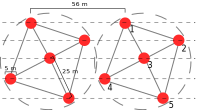
\includegraphics[width=0.8 \columnwidth]{lidar2img/fig/lola_shots.pdf}
	\caption{Two LOLA shots, part of a track. Each shot provides five
		distance measurements in a cross pattern. Shots are 56 m
		apart, and each laser beam reflects off a five meter diameter spot.}
	\label{fig:lolashots}
\end{figure}

The laser data is acquired from the Lunar Orbiter Laser Altimeter (LOLA), an instrument of the
Lunar Reconaissance Orbiter (LRO). The LOLA splits a laser into five parts to take five distance
measurements to the lunar surface, arranged in a cross shape. Each set of five measurements
is called a \emph{shot}. Each of the five laser beams
illuminates a 5 m diamter spot on the moon's surface (see Figure \ref{fig:lolashots}).

The LRO flies above the surface of the moon in a polar orbit, taking LOLA shots directly beneath
it as it moves.
Successive shots are approximately 56 m apart, and each sequence of shots from the same
orbit forms a \emph{track}. Figure \ref{fig:elevation} shows the elevation profile
of a crater as measured by two LOLA tracks.

